\documentclass{standalone}
\usepackage{tikz}
\usepackage{bm}
\renewcommand*\familydefault{\sfdefault}
\usepackage[italic]{mathastext}
\usepackage{isomath}

\begin{document}
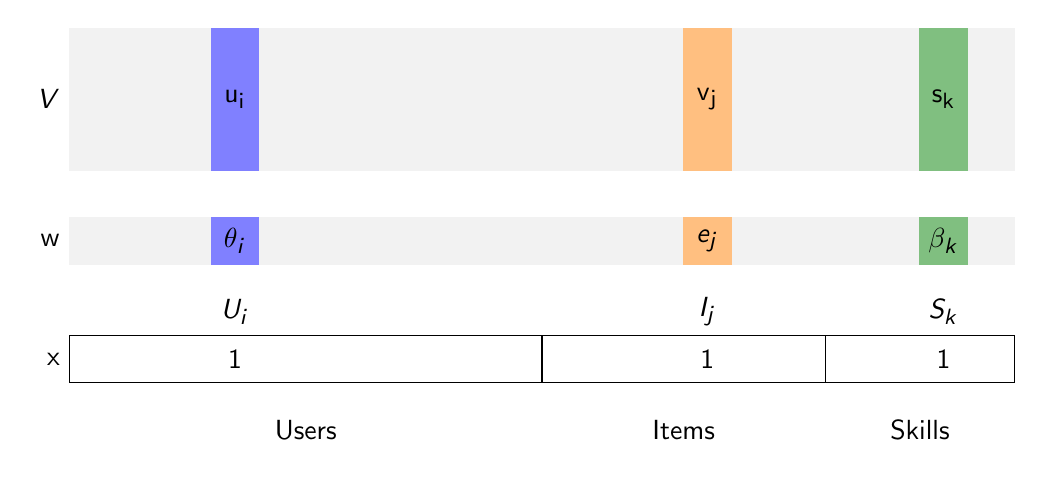
\begin{tikzpicture}[scale=0.6]
\filldraw[gray!10!white] (0,2.5) rectangle ++(20,1);
\filldraw[gray!10!white] (0,4.5) rectangle ++(20,3);
% LR
\filldraw[blue!50!white] (3,2.5) rectangle ++(1,1);
\filldraw[orange!50!white] (13,2.5) rectangle ++(1,1);
\filldraw[green!50!black!50!white] (18,2.5) rectangle ++(1,1);
% FM
\filldraw[blue!50!white] (3,4.5) rectangle ++(1,3);
\filldraw[orange!50!white] (13,4.5) rectangle ++(1,3);
\filldraw[green!50!black!50!white] (18,4.5) rectangle ++(1,3);

\draw (0,0) rectangle (20,1);
\draw node[left] at (0,0.5) {$\bm{x}$};
\draw node[left] at (0,3) {$\bm{w}$};
\draw node[left] at (0,6) {$V$};
\node at (3.5,0.5) {1};
\node at (3.5,3) {$\theta_i$};
\node at (3.5,6) {$\bm{u_i}$};
\node at (13.5,0.5) {1};
\node at (13.5,3) {$e_j$};
\node at (13.5,6) {$\bm{v_j}$};
\node at (18.5,0.5) {1};
\node at (18.5,3) {$\beta_k$};
\node at (18.5,6) {$\bm{s_k}$};
\node at (3.5,1.5) {$U_i$};
\node at (13.5,1.5) {$I_j$};
\node at (18.5,1.5) {$S_k$};

\draw (10,0) -- ++(0,1);
\draw (16,0) -- ++(0,1);
\node at (5,-1) {Users};
% \node at (5,4) {$\theta$};
\node at (13,-1) {Items};
\node at (18,-1) {Skills};
% \node at (13,4) {$-d$};
\end{tikzpicture}
\end{document}
